\section*{Dati e risultati}

\subsection*{Flip-Flop SR}

Il primo circuito che andiamo ad analizzare è un Flip-Flop SR, anche noto in letteratura come Latch SR. Questo è il Flip-Flop più semplice da realizzare.
Il suo schema circuitale è riportato in Figura \ref{fig:latch}. Possiamo notare che è stato realizzato sfruttando solo quattro porte NAND.
Quello che abbiamo fatto è stato collegare le due uscite $Q$ e $\overline{Q}$ alla schedina LED in modo che si potesse visualizzare l'uscita in funzione della tensione dei due ingressi S ed R (\SI{+5}{\volt} o \SI{0}{\volt}). Ricordiamo che S ed R stanno per Set (imposta) e Reset (reimposta).
A questo punto vogliamo verificarne il funzionamento. Abbiamo ottenuto il seguente risultato:

\begin{table}[h]
    \centering
    \begin{tabular}{llll|ll}
	\toprule
		S & R & $\overline{S}$ & $\overline{R}$ & Q & $\overline{Q}$ \\
	\midrule
		0 & 0 & 1 & 1 & x & y \\
		0 & 1 & 1 & 0 & 0 & 1 \\
		1 & 0 & 0 & 1 & 1 & 0 \\
		1 & 1 & 0 & 0 & 1 & 1 \\
	\bottomrule
	\end{tabular}
    \caption{Tabella di verità del circuito in Figura \ref{fig:latch}. S ed R sono gli ingressi, mentre q e $\overline{Q}$ sono le uscite del circuito elettronico.}
    \label{tab:latch}
\end{table}

La Tabella \ref{tab:latch} mostra l'andamento di $Q$ e $\overline{Q}$ in funzione del valore di tensione assunto dagli ingressi S e R. Come è possibile osservare quando S e R si trovano alternativamente ai valori logici 0 e 1 le uscite hanno valore corrispondente agli ingressi ad esse collegati.
Nel momento in cui entrambi gli ingressi si trovano allo stato 1 logico le uscite assumono entrambe valore 1. Invece nel momento in cui entrambi gli stati di ingresso si trovano allo 0 logico le uscite rimangono con gli stessi valori logigi della configurazione precedente.
Quindi se S = 1 e R = 0 abbiamo che Q = 1 e $\overline{Q}$ = 0 e portando S a 0 le uscite rimangono invariate. Mentre se si parte con S = 0 e R = 1 quindi Q = 0 e $\overline{Q}$ = 1 e si commuta R a 0 le uscite rimangono a 0 e 1 rispettivamente. Pertanto possiamo osservare, escludendo la situazione in cui entrambi gli ingressi si trovano ad 1 logico, che variando semplicemente 1 solo dei due stati in ingresso la situazione rimane immutata, ma nel momento che i valori in ingresso vengono variati entrambi, quindi passando da 1 e 0 a 0 ed 1 anche i valori in uscita variano di conseguenza. Quindi a meno che non si cambi la tensione ai capi di entrambi gli ingressi, il dispositivo memorizza lo stato in cui si trova.

\subsection*{Flip-Flop SR Sincronizzato}

Questo dispositivo è una variante dl dispositivo visto in precedenza. Il suo schema ciruitale è riportato in Figura \ref{fig:syncro}. Come è possibile osservare dalla Figura \ref{fig:syncro} l'unica variazione rispetto al caso precedente è quella di aver collegato i pin numero due di entrambe le porte NAND di S e R al generatore di funzioni d'onda. Quindi entrambi gli ingressi ricevono un'onda quadra in ingressodi ampiezza \SI{5}{\volt} picco picco con un offset di \SI{2.5}{\volt} e una fraquenza variabile. La frequenza in ingresso è detta di clock. A questo punto siamo andati a verificarne il funzionamento e abbiamo il seguente risultato (Tabella \ref{tab:syncro})

\begin{table}[h]
    \centering
    \begin{tabular}{llcll|ll}
	\toprule
		S & R & CLK & $\overline{S}$ & $\overline{R}$ & Q & $\overline{Q}$ \\
	\midrule
		0 & 0 & 1 & 1 & 1 & x & y \\
		0 & 1 & 1 & 1 & 0 & 0 & 1 \\
		1 & 0 & 1 & 0 & 1 & 1 & 0 \\
		1 & 1 & 1 & 0 & 0 & 1 & 1 \\
	\bottomrule
	\end{tabular}
    \caption{Tabella di verità del circuito in Figura \ref{fig:syncro}. S ed R sono gli ingressi, mentre q e $\overline{Q}$ sono le uscite del circuito elettronico. CLK è il segnale di clock fornito dal generatore di forme d'onda.}
    \label{tab:syncro}
\end{table}

Nella Tabella \ref{tab:syncro} abbiamo indicato con CLK il segnale in ingresso dal generatore di forme d'onda. Lo abbiamo espresso mediante i valori di verità 1 e 0. Possiamo notare come, in Tabella \ref{tab:syncro}, sia riportata solo al situazione in cui il segnale di clk è ad 1 logico. Questo è motivato dal fatto che se clk si trovasse allo 0 logico gli ingressi sarebbero disabilitati e $\overline{S}$ e $\overline{R}$ si troverebbero entrambi ad 1 logico e quindi le uscite Q e $\overline{Q}$ sarebbero in uno stato non ben definito che indichiamo con x e y rispettivamente, come nella sezione precedente. Al contrario quando clk è ad 1 logico gli ingressi S e R sono abilitati e pertanto si ricade nella trattazione della sezione precedente.

Quindi possiamo dire che il segnale di clk serve per abilitare o meno la scrittura sul nostro dispositivo. Quando clk è basso anche variando i valori di S e R non si varia il valore delle uscite. Questo è un vantaggio dal momento che con clk ad 1 logico io posso settare le uscite in una delle due configurazioni (1-0 o 0-1) ome visto nella sezione precedente. In seguito portando clk allo 0 logico, anche variando i valori di S e R io non vario il valore delle uscite del mio dispositivo. Quindi ho uno strumento di memoria.  

\subsection*{Flip-Flop SR D-Type}

Il Flip-Flop SR D-Type è il dispositivo che maggiormente approssima il concetto di memoria che abbiamo. Ovvero un dispositivo elettronico che se abilitato assume valore logico 1 o 0 e una volta disabilitato lo mantiene. Lo schema circuitale di questo FF SR D-Type è rappresentato in Figura \ref{fig:d-type}.
Quindi anche di questo circuito andiamo ad analizzarne la tabella di verità:

\begin{table}[h]
    \centering
    \begin{tabular}{lc|ll}
	\toprule
		A & CLK & Q & $\overline{Q}$ \\
	\midrule
		0 & 1 & 0 & 1 \\
		0 & 1 & 1 & 0 \\
		x & 0 & y & z \\
	\bottomrule
	\end{tabular}
    \caption{Tabella di verità del circuito in Figura \ref{fig:syncro}. A rappresenta l'input del circuito e CLK è il segnale di clock.}
    \label{tab:d-type}
\end{table}

Nella Tabella \ref{tab:d-type} possiamo notare che quando ilsegnale di clk è a 0 logico allora la scrittura è disabilitata e quindi l'uscita del dispositivo non è ben definita (y e z) nonostante in ingresso ci possa essere sia 1 che 0. Al contrario nel momento in cui clk è ad 1 logico la srittura è abilitata e quindi a seconda del valore di A che dò in ingresso in uscita (Q) avrò una replica di questo valore. Naturalmente per l'uscita $\overline{Q}$ il valore logico sarà il negato di Q.
Quindi come è possibile intuire questo circuito memorizza l'ingresso dato se clk = 1 e una volta disabilitato clk = 0, anche variando il valore di A, non cambiano i valori di uscita del circuito.

\subsection*{Antirimbalzo}

In questa sezione andremo a studiare e a capire il funzionamento del circuito realizzato in Figura \ref{fig:rimbalzo}.
La tabella di verità che abbiamo ricavato per questo circuito è la seguente:

\begin{table}[h]
    \centering
    \begin{tabular}{ll|ll}
	\toprule
		S & R & Q & $\overline{Q}$ \\
	\midrule
		0 & 0 & 1 & 1 \\
		0 & 1 & 1 & 0 \\
		1 & 0 & 0 & 1 \\
		1 & 1 & x & y \\
	\bottomrule
	\end{tabular}
    \caption{Tabella di verità del circuito in Figura \ref{fig:rimbalzo}. S e R sono rispettivamente i valori di tensione assunti dagli ingressi del circuito. Dipendono dalla posizione dell'interruttore. Q e $\overline{Q}$ sono i valori di uscita del circuito.}
    \label{tab:rimbalzo}
\end{table}

Nella Tabella \ref{tab:rimbalzo} è illustarto il comportamento del nostro circuito a seconda dei valori di tensione assunti dai due ingressi S e R. Aiutandoci sia con la Figura \ref{fig:rimbalzo} che con la Tabella \ref{tab:rimbalzo} possiamo notare come entrambi gli ingressi siano collegati ad una tensione di \SI{+5}{\volt} mediante una resistenza da \SI{1}{\kilo\ohm}. Quindi, a seconda della posiszione dell'interruttore, la tensione ai capi di un ingresso può essere alta (\SI{+5}{\volt}) o bassa (\SI{0}{\volt}). Naturalmente nel momento in cui un ingresso è ad alta tensione l'altro si troverà a bassa tensione, in quanto siamo al cospetto di un interruttore. Quindi della Tabella \ref{tab:rimbalzo} le configurazioni possibili sono quelle per cui S e R assumono rispettivamente valori 0-1 o 1-0.

Su questo circuito abbiamo sperimentato due tipi differenti di interruttore. Il primo è un interruttotre con lamina. Abbiamo analizzato sull'oscilloscopio l'uscita Q del circuito per capire come si comportasse l'interruttore con lamina. Abbiamo trovato il risultato riportato in Figura \ref{fig:rimbalzo_lamina_plot}.

Possiamo notare che la tensione ai capi di Q prima di stabilizzarsi ci impiega circa \SI{200}{\micro\second}. Queste fluttuazioni sono dovute ai rimbalzi della lamina dell'interruttore contro il contatto del circuito che provocano l'oscillazione del segnale in igresso e dunque anche di quello in uscita tra le tensioni di \SI{+5}{\volt} e \SI{0}{\volt}.

Abbiamo fatto lo stesso tipo di misura per un interruttore del tipo a molla. Il risultato trovato e riportato in Figure \ref{fig:rimbalzo_molla_plot}.

Quello che possiamo osservare è che:

Infine mantnendo la stessa configurazione circuitale fatta eccezione per l'interruttore, sostituito grezzamente con due cavi collegati direttamente a massa, possiamo manipolare la tensione ai capi dei due ingressi sfruttando due cavetti mobili che connettiamo manualmente con i cavetti a massa.
Quello che abbiamo ottenuto è un funzionamento analogo a quello riscontrato per il circuito in Figura \ref{fig:rimbalzo}.
L'unica variante che otteniamo e che i due ingressi possono avere lo stesso valore logico. Quindi in questo caso la tabella di verità é esattamente la Tabella \ref{tab:rimbalzo} con tutte e quattro le combinazioni di S e R possibili. 

\subsection*{Divisore di frequenza}

In questa ultima sezione vogliamo analizzare un divisore di frequenze. Se ci si pensa bene, già di per sè non è compito semlice realizzare un dispositivo che moltiplichi per un nuero intero positivo una frequenza, figuriamoci un dispositico che ne fraziona una data!
Ebbene grazie al dispositivo Flip-Flop è possibile fare anche questa operazione. In particolare andiamo a realizzare un divisore di frequenze, ovvero un dispositivo che restituisce in uscita un segnale che ha una frequenza dimezzata rispetto a quello in ingresso.
Il circuito che ci permette di fare questa operazione è raffigurato in Figura \ref{fig:divisore}. Questo circuito è realizzato a partire da un circuito integrato SN74LS109 a 16 pin che racchiude due FF JK Toggle.

Al fine di capire come in uscita si possa ottenere una frequenza che è la metà rispetto a quella in ingresso dobbiamo spendere alcune parole per il Flip-Flop JK Toggle. Questo particolare tipo di FF ha la caratteristica che fissati i valori dei due ingressi J e K come 0-1 o 1-0 rispettivamente, sfruttando il segnale di clk, il dispositivo, solo sul fronte di discesa del segnale, fa cambiare stato alle uscite. In particolare inverte i valori di Q e $\overline{Q}$. Quindi dato un segnale di clock, le oscillazioni del segnale in uscita saranno scandite solo dal fronte in discesa dell'impulso di clk, quindi la frequenza in output risulta essere la metà di quella in in ingresso. Questo perchè tra due fronti di discesa di clk, che sono l'ampiezza dell'oscillazione di outpu, si hanno due cicli del segnale di clock.

Pertanto se si mettono semplicemente a cascata due o più FF JK Toggle si possono dividere le frequenze per un fattore che corrisponde a $2^n$ con $n$ che indica il numero di dispositivi messi in cascata. Quindi se la frequenza di clock vale $f_0$ in base a quanti FF JK Toggle vengono posti in cascata possiamo ottenere il seguente risultato:
\begin{equation}
	f_n\,=\,\frac{f_0}{2^n}
\end{equation}
dove $f_n$ rppresenta la frequenza in uscita dal circuito.

Quindi nel nostro caso abbiamo ottenuto il seguente risultato, illustrato nel rafico in Figura \ref{fig:divisore_plot}

%\begin{wrapfloat}{table}{I}{300pt}
%\centering
%	\begin{tabular}{l | llll | l}
%	\toprule
%		In & A & B & C & D & Out\\
%	\midrule
%		1 & 0 & 1 & 0 & 1 & 1 \\
%		0 & 1 & 0 & 1 & 0 & 1 \\
%	\bottomrule
%	\end{tabular}
%	\caption{Tabella di verità del circuito in Figura \ref{fig:ritardo}}
%	\label{tab:ritardo}
%\end{wrapfloat}

%\begin{wrapfloat}{figure}{I}{0pt}
%\includegraphics[width=0.5\textwidth]{Relativo}
%\caption{Esempio di figura ‘‘avvolta’’ da un testo.}
%\end{wrapfloat}

%\begin{center}
%	\begin{tabular}{lll}
%	\toprule
%		A & B & C \\
%	\midrule
%		& & \\
%		& & \\
%		& & \\
%		& & \\
%	\bottomrule
%	\end{tabular}
%\end{center}

%\begin{figure}[t!]
%    \centering
%    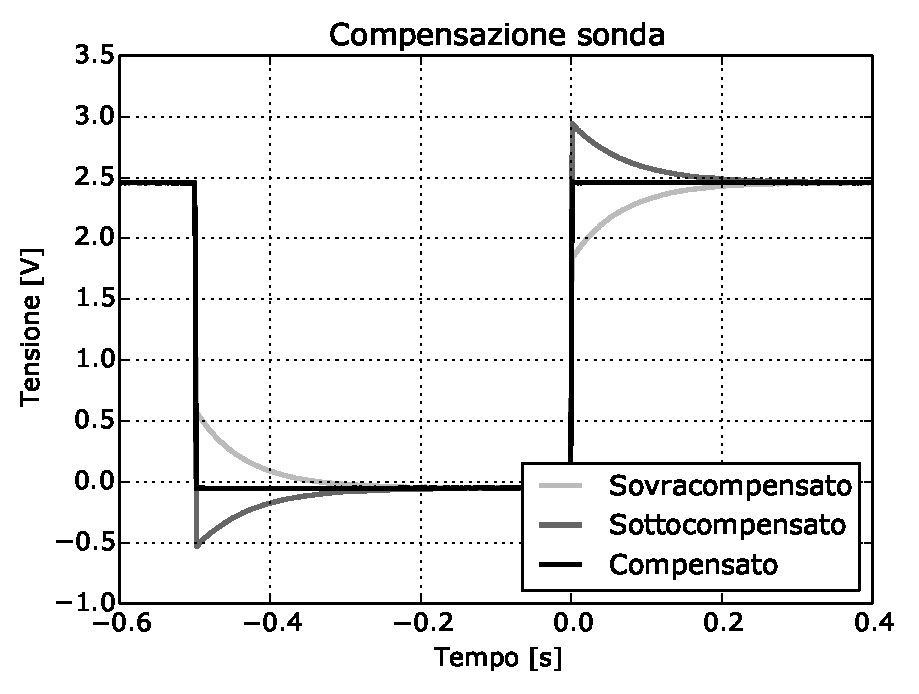
\includegraphics[width=\columnwidth]{figure/comp.pdf}
%    \caption{Input dell'oscilloscopio con una sonda compensabile. Cambiando capacità
%        si può ottenere una sottocompensazione, una sovracompensazione oppure compensare perfettamente
%        le capacità, ottenendo un'onda quadra.}
%    \label{fig:compensazione}
%\end{figure}

%\begin{wrapfloat}{figure}{O}{0pt}
%        \def\svgwidth{0.4\textwidth}
%        \subimport{figure/}{raddrizzatore.pdf_tex}
%        \caption{Raddrizzatore di precisione a semionda. Alimentato, inizialmente con una $V\ped{in}\,=\,\SI{1.02}{\volt}$ di frequenza $\nu\,=\,\SI{50}{\hertz}$.}
%        \label{fig:radd}
%\end{wrapfloat}

%\begin{SCfigure}[][p]
%        \centering
%        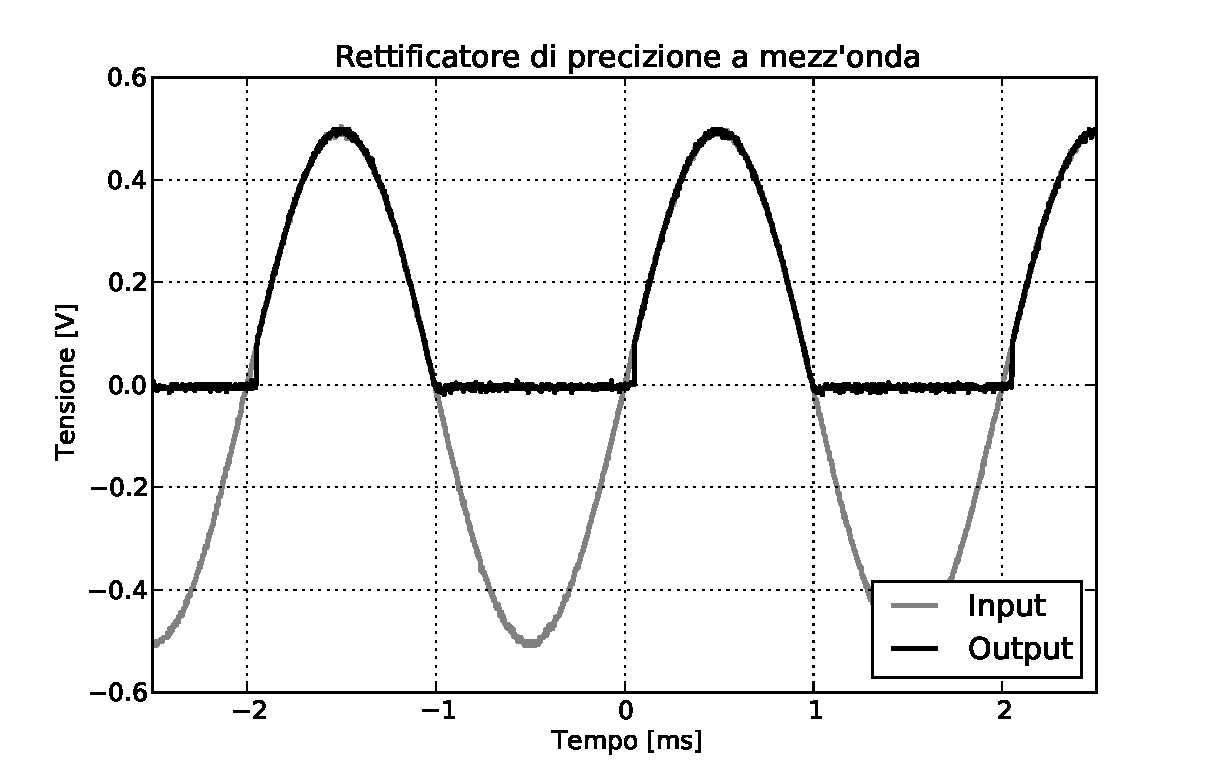
\includegraphics[width=0.7\textwidth]{figure/rett.pdf}
%        \caption{Questo grafico illustra l'andamento di $V\ped{out}$, linea nera, in funzione di $V\ped{in}$, linea grigia. Si nota chiaramente, come da previsioni, che la parte negativa del segnale in ingresso impediscse al diodo di condurre, pertanto la tensione di output risulta nulla. Inoltre, come si può osservare, il fronte di salita di $V\ped{out}$ presenta un leggero ritardo rispetto al segnale in ingresso $V\ped{in}$. Questo ritardo è stato stimato essere approssimativamente di circa $(152\pm10)\SI{}{\micro\second}$.}
%        \label{fig:radd_plot1}
%\end{SCfigure}
